\begin{itemize}
    \item Principal Component Analysis (PCA) is a dimension-reduction tool.
    \item The first principal component accounts for as much of the variability in the data as possible, and each succeeding component accounts for as much of the remaining variability as possible.
    \item PCA seeks a linear combination of variables such that the maximum variance is extracted from the variables.
    Those PCs are the eigenvectors decomposed and eigenvalues determine weight of each PC.
    \item \textbf{Explained Variance is ratio of eigenvalues. (PC eigenvalue / summation of all eigenvalues)}
    \begin{figure}[H]
        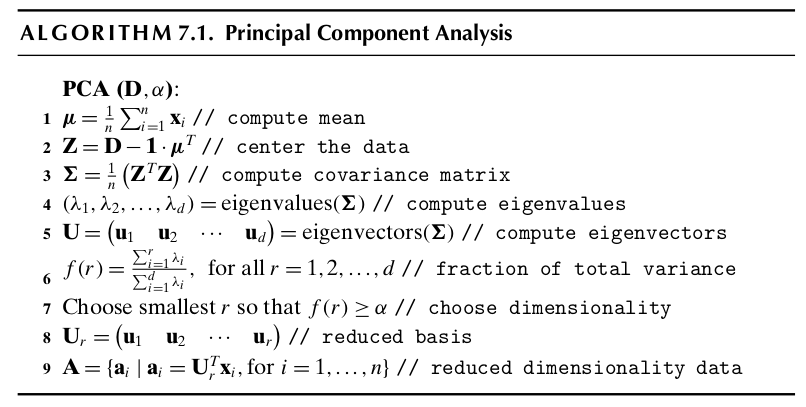
\includegraphics[width=\textwidth]{Figures/pca.png}
        \caption{\label{fig:figure1}PCA Algorithm}
    \end{figure}
\end{itemize}